\section{Filter Fun}
You're given the following filter, and you measure the magnitude and phase of
its transfer function ($H(j\omega) = \frac{V_o(j\omega)}{V_i(j\omega)}$) in the
lab, as shown in the following plots:

\begin{minipage}[l]{0.3\linewidth}
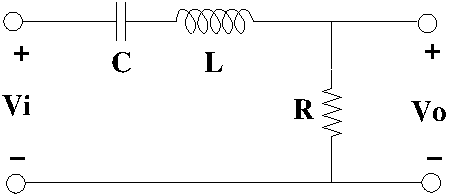
\includegraphics[width=1.0\linewidth]{bpf/bpf_ckt}
\end{minipage}\hfill
\begin{minipage}[l]{0.7\linewidth}
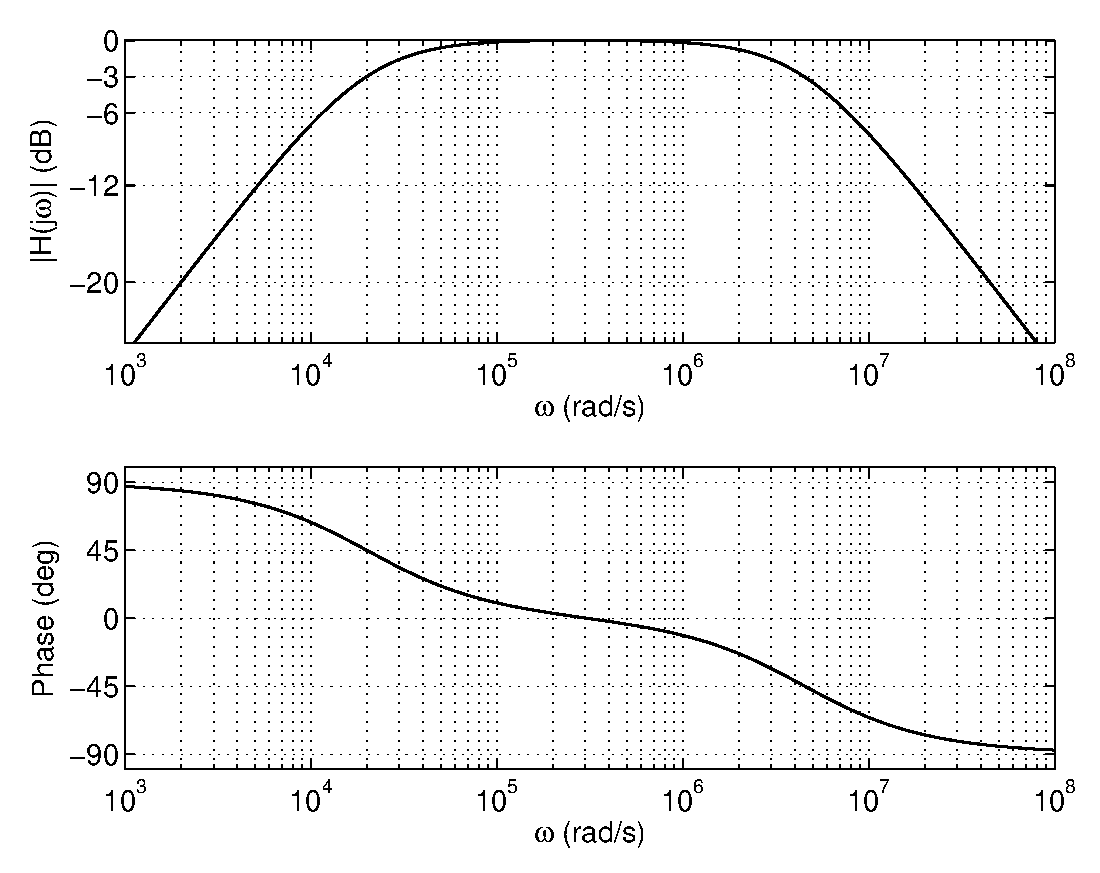
\includegraphics[width=1.0\linewidth]{bpf/bpf}
\end{minipage}

\begin{enumerate}
    \item What type of filter is this (specify whether it is first- or
    second-order)?  What is/are this filter's cutoff frequency/frequencies
    (reasonable estimates are okay)?

    \item If $V_i(t) = 0.5 \cos(2000t)$ V, then what is $V_o(t)$ (again, reasonable estimates are okay)?

    \item Solve for the values of $R$ \& $L$ needed to achieve this transfer
    function, assuming that $C$ = 5.55 nF and the quality factor for this circuit
    can be expressed as $Q = \frac{1}{R}\sqrt{\frac{L}{C}}$.
\end{enumerate}
